\section{Track Finding Processor Demonstrator and Results}\label{sec:tf-results}
\subsection{Demonstrator}
Simulated physics events with a \PU of up to 200 proton-proton interactions per bunch crossing have been run through the demonstrator system in order to measure and validate the performance, within the latency constraints, of a scalable slice of the Track Finder. As such, by sequentially running through each $\phi$ octant of the tracker across all $\eta$ for each time-multiplexed period, results for the entire tracking detector can be obtained.

The demonstrator consists of eight Imperial Master Processor Extended Edition (MP7-XE) double width AMC Boards \cite{mp7ref}, five for the entire TFP, two for the detector octant \textit{Sources} which inject up to thirty consecutive events, loaded directly from simulation via IPBus \cite{IPBus}, into the TFP, and a \textit{Sink} to buffer and store up to thirty events before being read-out again with IPBus. This demonstrator, located at the CERN Tracker Integration Facility (TIF), is installed in a custom dual-star MicroTCA \cite{uTCA} crate, which provides power and cooling, that is equipped with a commercial NAT MicroTCA Carrier Hub (MCH) for Gigabit Ethernet communication via the backplane, and a CMS specific auxiliary card known as the AMC13 \cite{AMC13} that provides synchronisation, timing and control.

The MP7 was considered to be an ideal solution for developing the system  as it was originally designed for the upgraded CMS L1 time-multiplexed calorimeter trigger, thus providing a well tested platform with existing infrastructure tools. As the tools are isolated from the algorithms within the firmware, a generic algorithm interface allows for the easy swapping of algorithms, reduced development time and the daisy-chaining of multiple firmware blocks on separate boards. 

%\begin{figure}[!t]
%\centering
%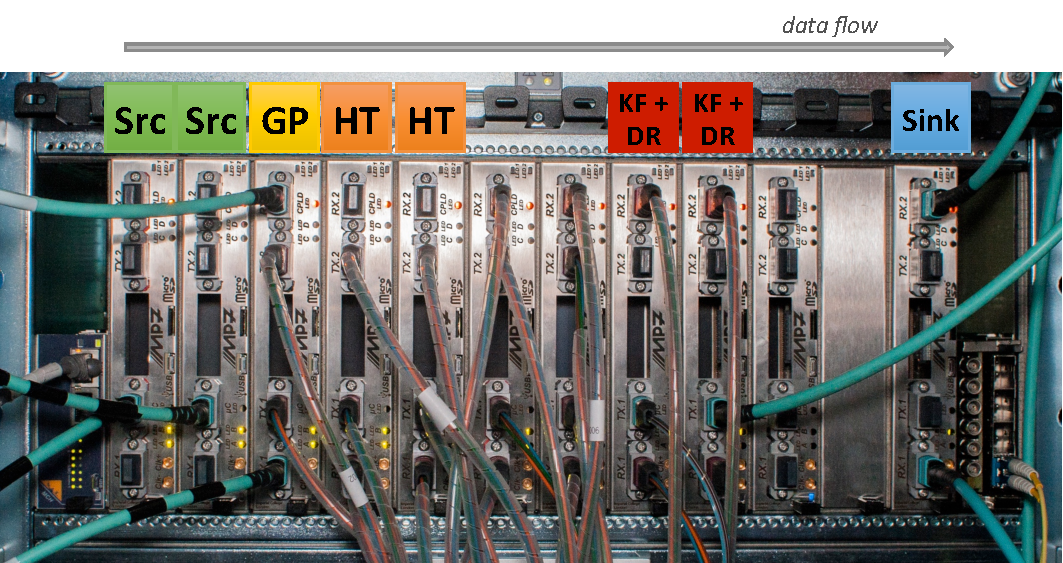
\includegraphics[width=5in]{figs/demoslice/democrate.pdf}
%% where an .eps filename suffix will be assumed under latex,
%% and a .pdf suffix will be assumed for pdflatex; or what has been declared
%% via \DeclareGraphicsExtensions.
%\caption{The demonstrator system crate at the CERN Tracker Integration Facility, consisting of %eleven MP7-XE boards (three of which are spare), an AMC13, MCH and the connecting optical links.
%}
%\label{Demonstrator}
%\end{figure}

\subsection{Results}
\subsubsection{Track Reconstruction Efficiency}

Track reconstruction efficiency is measured relative to all generated charged particles from the primary interaction which produce stubs in at least four layers of the tracker and lie within the kinematic acceptance range of: \pt > 3\GeV; $|\eta| < 2.4$; $|z_{0}|<30$\cm; $|L_{xy}|<1$\cm (where $L_{xy}$ is the distance between the beam line to the particle's vertex in the transverse plane.

For charged particles which meet this criteria, they are deemed to have been successfully matched if the reconstructed track contains stubs from at least four different tracker layers and all stubs are generated by that particle.

Tracks from charged particles which do not meet this definition are known as \textit{fake tracks	}. If more than one track matches to a charged particle, the additional tracks are considered to be \textit{duplicate tracks}.

Excellent agreement between hardware and emulation has been measured for the full chain in \ttbar events with 200 \PU, as shown in Fig.~\ref{fig:ttbarEffPlots}. Identical performance is observed for the emulator for both floating-point and integer precision stub data.

Whilst there is excellent reconstruction efficiency for muons in the \ttbar events electron reconstruction efficiency is, as expected, lower (Fig.~\ref{fig:leptonEffPlots}. This is mainly due to bremsstrahlung effects, resulting in the particle deviating from the helix assumed. It is expected however, that some lost efficiency should be recoverable by modifying the \KF to account for multiple scattering.

\begin{figure}[!t]
\centering
\includegraphics[width=0.47\textwidth]{figs/tk-results/EfficiencyVsPt1800evttbar200pu.pdf}
\hfill
\includegraphics[width=0.47\textwidth]{figs/tk-results/EfficiencyVsEta1800evttbar200pu.pdf}
% where an .eps filename suffix will be assumed under latex,
% and a .pdf suffix will be assumed for pdflatex; or what has been declared
% via \DeclareGraphicsExtensions.
\caption{Track reconstruction efficiency for inclusive \ttbar events at 200 \PU as a function of \pt (left) and $\eta$ (right).}
\label{fig:ttbarEffPlots}
\end{figure}

\begin{figure}[!t]
\centering
\includegraphics[width=0.47\textwidth]{figs/tk-results/TTbar_eff_pt_Leptons.pdf}
\hfill
\includegraphics[width=0.47\textwidth]{figs/tk-results/TTbar_eff_eta_Leptons.pdf}
% where an .eps filename suffix will be assumed under latex,
% and a .pdf suffix will be assumed for pdflatex; or what has been declared
% via \DeclareGraphicsExtensions.
\caption{Track reconstruction efficiency for muons and electrons in \ttbar events at 200 \PU as a function of \pt (left) and $\eta$ (right).}
\label{fig:leptonEffPlots}
\end{figure}

\subsubsection{Track Parameter Resolution}
There is a reasonable level of agreement between hardware and emulation for the resolution of the four track parameters ($\pt, \phi, \cot{\theta}, z_0$) for reconstructed tracks from \ttbar events at pileup 200. The use of floating-point maths in the emulator code accounts for the differences between hardware and emulation. 

The resolution of the four parameters compares well with offline simulation \cite{CMS_Upgrade_TP}, which is able to make use of all available information from the tracking system and more sophisticated software reconstruction algorithms. Whilst the \pt and $\phi$ resolution measured in the demonstrator is comparable to offline performance, the other two parameters are an order of magnitude coarser due to the offline reconstruction being able to make use of tracking information from the pixel detector.

\begin{figure}[!t]
\centering
\includegraphics[width=0.47\textwidth]{figs/tk-results/ptresoverpt-ttbar-200pu-1800ev.pdf}
\includegraphics[width=0.47\textwidth]{figs/tk-results/phi0resolutionVsEta1800evttbar200pu.pdf}
\includegraphics[width=0.47\textwidth]{figs/tk-results/z0resolutionVsEta1800evttbar200pu.pdf}
\includegraphics[width=0.47\textwidth]{figs/tk-results/tanlresolutionVsEta1800evttbar200pu.pdf}
% where an .eps filename suffix will be assumed under latex,
% and a .pdf suffix will be assumed for pdflatex; or what has been declared
% via \DeclareGraphicsExtensions.
\caption{Relative \pt resolution, $\phi$ resolution[rad], $z_0$[\cm] and $\cot{\theta}$ resolution measured for tracks originating from the primary interaction point for \ttbar at \PU of 200 for both hardware and emulation.}
\label{fig:resolutionPlots}
\end{figure}

\subsubsection{FPGA Resource Usage}
Using multiple MP7 boards avoids the constraints of constructing a system on a single, current generation FPGA board. Table~\ref{tab:resourceusage} illustrates the total resource usage for the entire TFP and the resources available in several commercially available boards. It is not unreasonable to assume that the current TFP could fit onto either two Kintex Ultrascale 115 FPGAs or a single Ultrascale+ 11P FPGA. 

It is also worth noting that the resource usage of the system is smaller than that provided by the 5 Virtex 7s used to demonstrate the TFP. This is partly due to an over-engineered system designed to eliminate truncation effects, and as such, leads to wasted processing bandwidth. A factor of 4 reduction in resources required is anticipated to be feasible for the final system.

\begin{table}[!t]
\caption {Total resource usage for the demonstrator TFP, as implemented in the Xilinx Virtex-7 XC7VX690T FPGA \cite{virtexref}. The available resources for a number of commercial Xilinx FPGAs are shown for comparison \cite{ultrascaleRef}.}
\label{tab:resourceusage}
\centering
% This increases column spacing.
\addtolength{\tabcolsep}{0.5ex}
% This right-aligns numbers in column, but centers them under column title.
\begin{tabular}{lr@{\hspace{5.5ex}}r@{\hspace{2.5ex}}r@{\hspace{4.5ex}}r@{\hspace{5.5ex}}}
\hline
& \multicolumn{1}{r}{\bf{LUTs [$10 ^ 3$]}} & \multicolumn{1}{r}{\bf{DSPs}} & \multicolumn{1}{r}{\bf{FFs [$10 ^ 3$]}} & \multicolumn{1}{r}{\bf{BRAM} (36 Kb)} \\
\hline
\bf{GP}        & 121 & 1056 & 205  & 222 \\
\bf{HT}        & 244 & 2304 & 299 & 1188 \\
\bf{KF and DR} & 398 & 5112 & 316 & 1776 \\
\hline
\bf{Infrastructure per MP7} & 90 & 0 & 91 & 291\\
\hline
\bf{TFP Total (excl. infrastructure)} & 763 & 8472 & 820 & 3186 \\
%\bf{Max. per TFP for 18 BX TMP system (incl. infra)} & 1690 & 2900 & 6830 & 13200 \\
\hline
\hline
\bf{Virtex 7 690}           & 433  & 3600  & 866 & 1470 \\
\bf{Kintex Ultrascale 115}  & 633  & 5520 & 1266 & 2160 \\
\bf{Virtex Ultrascale+ 11P} & 1296 & 9216 & 2592 & 2016 \\
\hline
\end{tabular}
\addtolength{\tabcolsep}{-0.5ex}
\end{table}

\subsubsection{System Latency}
Latency measurements of full demonstrator chain have been measured for the each block independently and the entire chain - both give identical results, as shown in Table~\ref{tab:LatencyTable}. These measurements include optical link traversal time and serialisation/de-serialisation (SerDes). Latency of the entire system is fixed, regardless of pileup or event occupancy.

\begin{table}[!t]
\caption{Measured latency of the demonstrated components of the track reconstruction chain, including the serialisation/de-serialisation (SerDes) and optical transmission delays between each board. Both first track in and first track out and first track in and last track out latency definitions provided are of interest to the downstream L1 trigger.}
\label{tab:LatencyTable}
\centering
% This increases column spacing.
\addtolength{\tabcolsep}{1ex}
% This right-aligns numbers in column, but centers them under column title.
\begin{tabular}{lr@{\hspace{6ex}}}
\hline
\bf{System Latency} & \multicolumn{1}{r}{\bf{Latency} [ns]} \\
\hline
SerDes \& optical length 1 & 143 \\
Geometric Processor       & 251 \\
SerDes \& optical length 2 & 144 \\
\HT                       & 1025 \\
SerDes \& optical length 3 & 129 \\
\KF + \DR                 & 1658 \\
SerDes \& optical length 4 & 129 \\
\hline
\hline
Total: First out - First in & 3479 \\
Last out - First out & 225 \\
Total: Last out - First in & 3704 \\
\hline
\end{tabular}
\addtolength{\tabcolsep}{-1ex}
\end{table}

\subsubsection{System Robustness Studies}
A number of simulation studies were carried out to determine the robustness of the demonstrator system for adverse operating conditions, more ambitious operational conditions and alternative detector geometries.

\subsubsubsection{Cooling Loop Failures}

In a situation where a number of tracker modules fail and do not produce stubs, for example during a cooling loop failure, localised losses can be mitigated against by relaxing the minimum number of hit layers required to form a track candidate from five to four for the affected sub-sectors only. Not only is the lost efficiency recovered (Fig.~\ref{fig:RobustPlots}, but there is a negligible increase in data rate (Table.~\ref{tab:coolingLoopRate}).

\begin{table}[!t]
\caption{Mean number of tracks per event after the \HT for a module loss scenario, for tracks originating from the primary interaction in \ttbar events with 200 \PU.}
\label{tab:coolingLoopRate}
\centering
% This increases column spacing.
\addtolength{\tabcolsep}{1ex}
\begin{tabular}{ccc}
\hline
\bf{No module loss} & \multicolumn{2}{c}{\bf{With module losses}} \\
              & \bf{Before recovery} & \bf{After recovery} \\
\hline
330 & 304 & 347 \\
\hline
\end{tabular}
\addtolength{\tabcolsep}{-1ex}
\end{table}

\subsubsubsection{Lowering the minimum \pT threshold}

Lowering the minimum track \pT threshold from 3\GeV to 2\GeV was explored as the availability of tracking at lower \pT could potentially be useful to the L1 trigger. To do this, the GP parameters would modified in order to provide sufficient duplication in $\varphi$ and the HT \qpt columns increased by 50\% to reflect the increased \pT range without sacrificing the precision of the estimate. The increase in the \qpt range increases the required FPGA resources by 50\% and results in an increase in the data rate from the HT by a factor of 2.2. In order to mitigate against a loss of tracking efficiency in the range 2 < \pT < 2.7GeV, caused mainly by multiple scattering resulting in some stubs being found outside of their expected HT cell, the precision of the HT is degraded by a factor of two along both axes. It has been shown in simulation (Fig.~\ref{fig:RobustPlots}) this allows for some recovery of lost efficiency, at the cost of an additional 10\% increase in rate. Further improvements and optimisations to the HT and KF could also improve performance.

\begin{figure}[!t]
\centering
\includegraphics[width=0.47\textwidth]{figs/tk-results/TTbar_eff_eta_CoolingLoop.pdf}
\hfill
\includegraphics[width=0.47\textwidth]{figs/tk-results/TTbar_eff_pT_2Gev.pdf}
% where an .eps filename suffix will be assumed under latex,
% and a .pdf suffix will be assumed for pdflatex; or what has been declared
% via \DeclareGraphicsExtensions.
\caption{Track reconstruction efficiency for tracks originating from the primary interaction in
tt events with 200 PU for the scenarios of a cooling loop failure (left) and for when the minimum \pt threshold is lowered to 2 GeV (right) as a function of $\eta$ and $1/\pt$ respectively.}
\label{fig:RobustPlots}
\end{figure}
